\subsection{Original Implementation} In the original BPMax implementation, all the diagonal elements are computed simultaneously, exposing the maximum level of parallelism. It accesses all the inner triangles  (highlighted in light red) towards the left of the diagonal points (red points Figure~\ref{fig:bpmax_original_schedule}). 
So, the total amount of the active data footprint required to compute all these points simultaneously can exceed the last-level cache for a larger input size, triggering a lot of data movement between different levels of caches and main memory. Memory reuse is almost impossible as we move to the next diagonal. Thus, the original program suffers from poor data locality.
\begin{figure}[htb]
\centerline{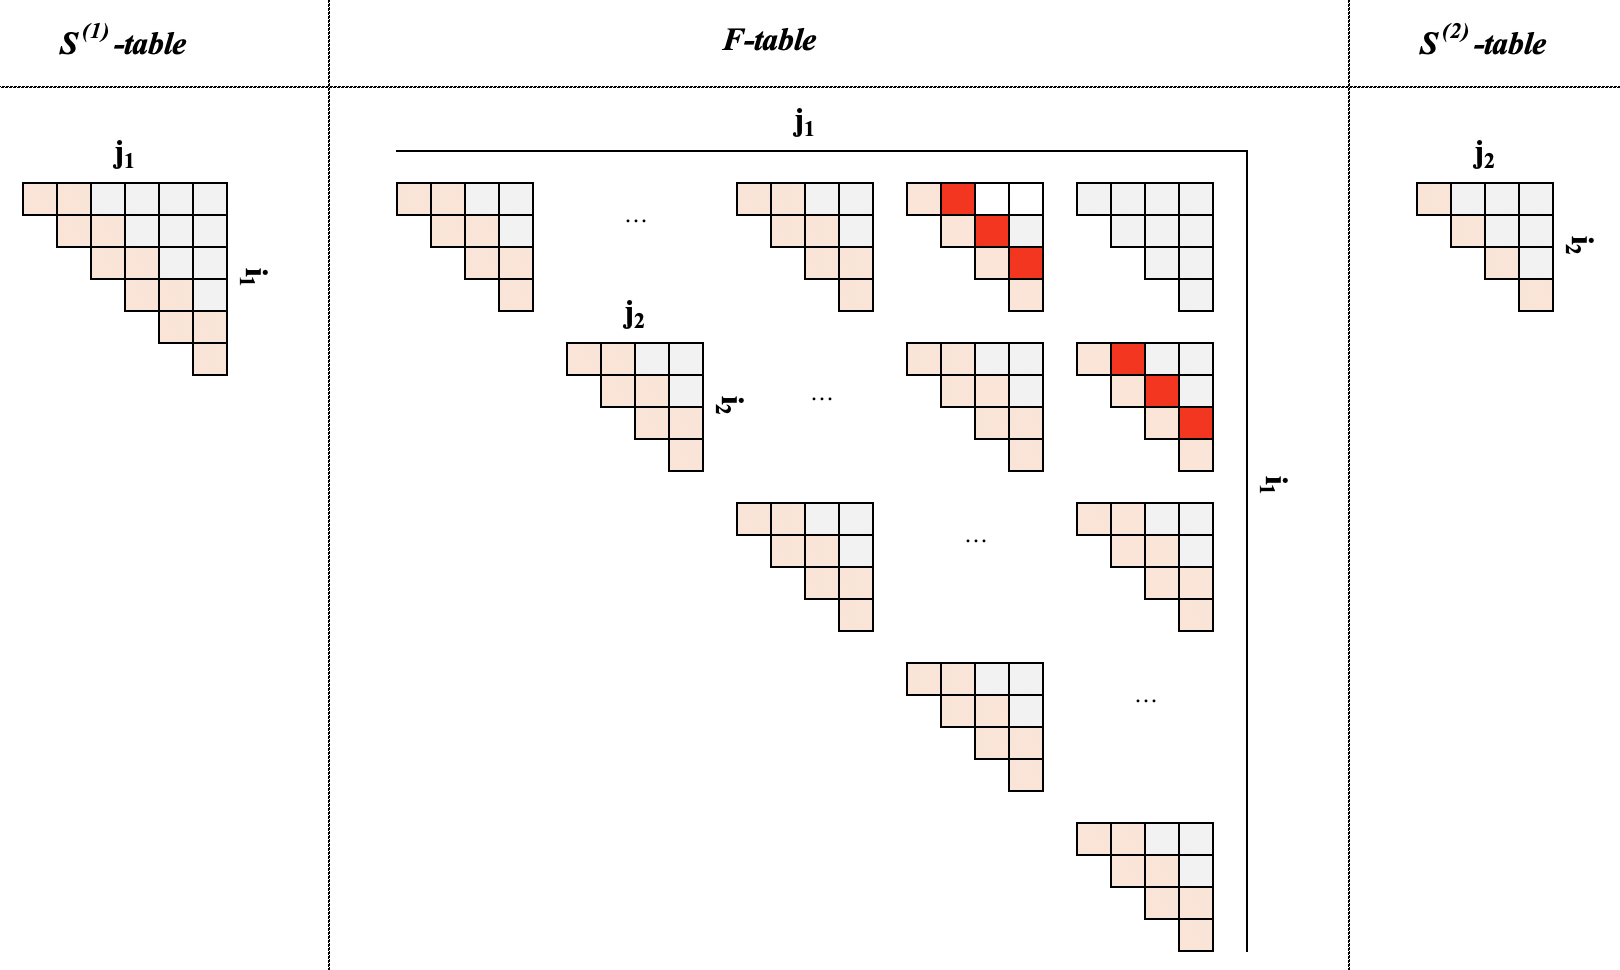
\includegraphics[scale=.30]{content/figures/bpmax_original_schedule.png}}
\caption{BPMax Original Schedule}
\label{fig:bpmax_original_schedule}
\end{figure}
Also, each of these reductions in the original implementation has loop carried dependencies, which prevents vectorization.

\subsection{Previous Optimization Approach} Our previous paper \cite{Mondal2021} introduced two levels of tiling to the BPMax - the first-level tilling to calculate each inner triangle at a time to improve the data locality. We also decomposed the double max-plus similar to \cite{Varadarajan2016} into a sequence of multiple matrix max-plus instances and applied loop tiling as the second-level tiling on each of the instances highlighted in Figure~\ref{fig:double_max_plus_accumulation_sequence_0}.
\begin{figure}[htbp]
\centering
\begin{subfigure}[b]{0.48\textwidth}
\centering
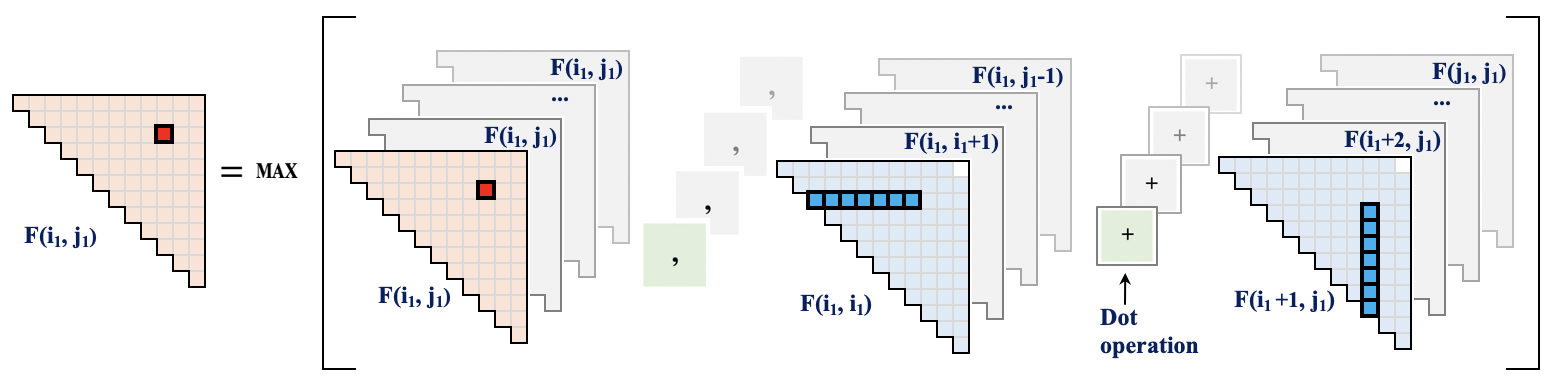
\includegraphics[scale=0.30, trim=4 4 4 4,clip]{content/figures/r0_1.png}
\caption{Decomposition of $R^{0}$}
\label{fig:double_max_plus_accumulation_sequence_0}
\end{subfigure}
\begin{subfigure}[b]{0.48\textwidth}
\vspace{1mm}
\centering
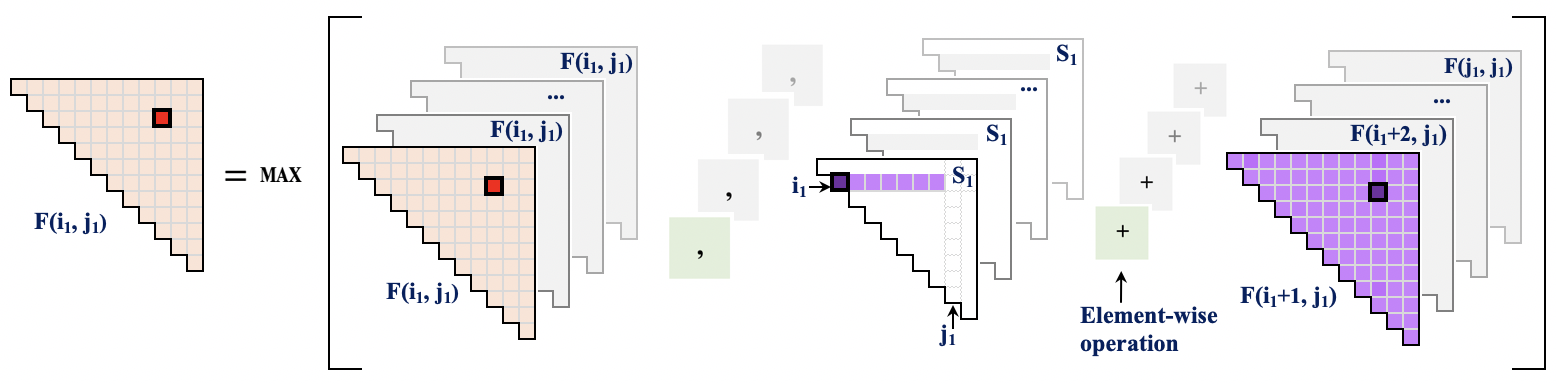
\includegraphics[scale=0.30, trim=4 4 4 4,clip]{content/figures/r3_1.png}
\caption{Decomposition of $R^{3}$}
\label{fig:R_3_optimization}
\end{subfigure}
\begin{subfigure}[b]{0.48\textwidth}
\vspace{1mm}
\centering
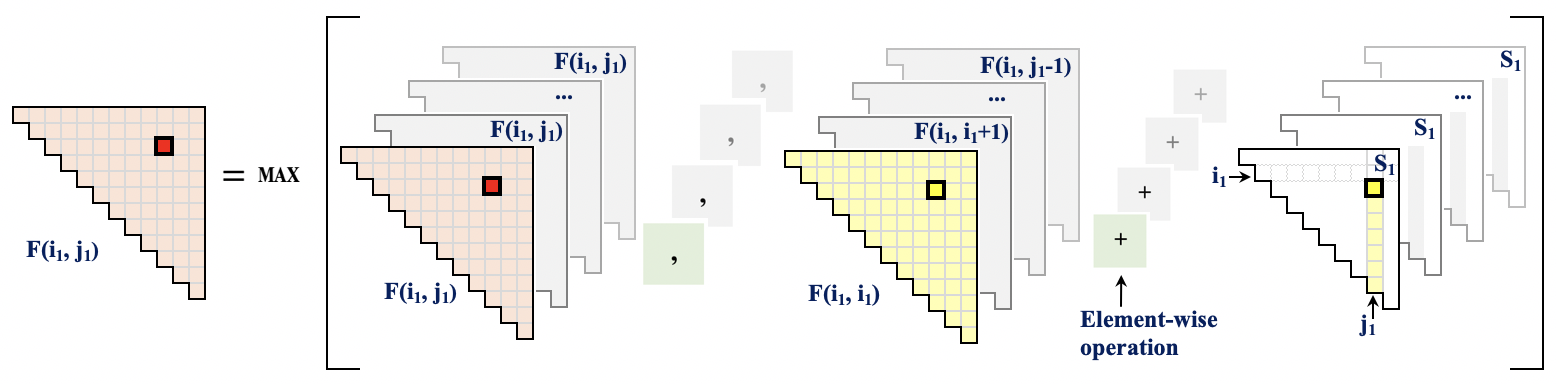
\includegraphics[scale=0.30, trim=4 4 4 4,clip]{content/figures/r4_1.png}
\caption{Decomposition of $R^{4}$}
\label{fig:R_4_optimization}
\end{subfigure}
\caption{$R^{0}$, $R^{3}$, and $R^{4}$ Accumulation}
\label{fig:bpm_outer_accumulation_sequence}
\end{figure}
We were able to tile each instance since there is no dependency between the input and output matrices. However, this approach had a few issues when we attempted to take advantage of auto-vectorization. It performed better only when the innermost dimension (vector dimension) was longer, which effectively prohibited the smaller tile dimension reducing better data locality. We noticed that $R^3$ requires the same inner triangles towards the south of $F(i_{1}, j_{1})$ and $S^{(1)}$, whereas $R^4$ requires the same inner triangles towards the west of $F(i_{1}, j_{1})$ and $S^{(1)}$ highlighted in Figure~\ref{fig:bpmax_dependency}. To take advantage of the re-use, we decomposed the $R^3$ similar to $R^0$ as a set of max-plus operations between $F$-table entries
(\{$F(k_{1}+1, j_{1}) \mid  i_{1} <=k_{1} < j_{1}$\}) 
and $S^{(1)}$ highlighted in Figure~\ref{fig:R_3_optimization}.
\begin{figure}[htbp]
\centering
\begin{subfigure}[htbp]{1\linewidth}
\centering
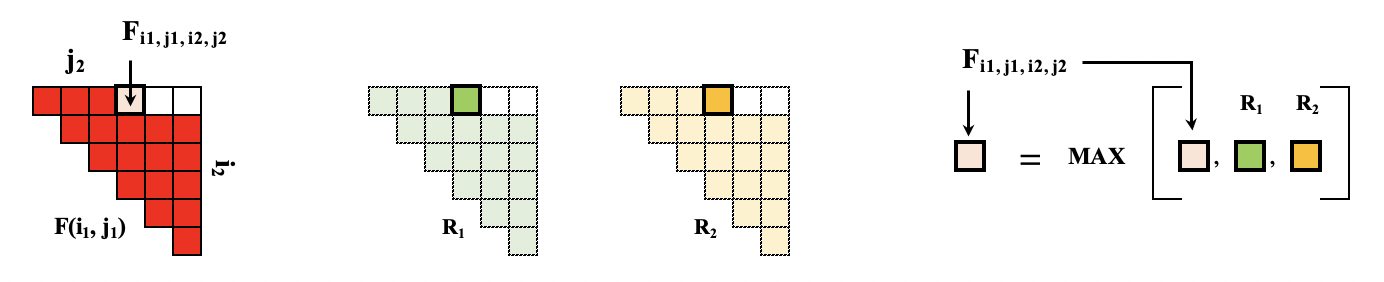
\includegraphics[scale=0.35, trim=4 4 4 4,clip]{content/figures/r0_r1_1.png}
\caption{Step 1: Let us assume that we are about to update the next element of $F(i_{1}, j_{1})$: $F_{i_{1}, j_{1}, i_{2}, j_{2}}$. Results of $R^{0}$, $R^{3}$, and $R^{4}$ corresponding to all the elements of $F(i_{1}, j_{1})$ are already accumulated in $F(i_{1}, j_{1})$. Let us also assume that  $R^{1}$ and $R^{2}$ are also computed for $F_{i_{1}, j_{1}, i_{2}, j_{2}}$ element. Thus, it gets updated with the maximum of the $F_{i_{1}, j_{1}, i_{2}, j_{2}}$,  $R^{1}$, and $R^{2}$.}
\label{fig:r3_r4_1}
\end{subfigure}
\begin{subfigure}[htbp]{1\linewidth}
\centering
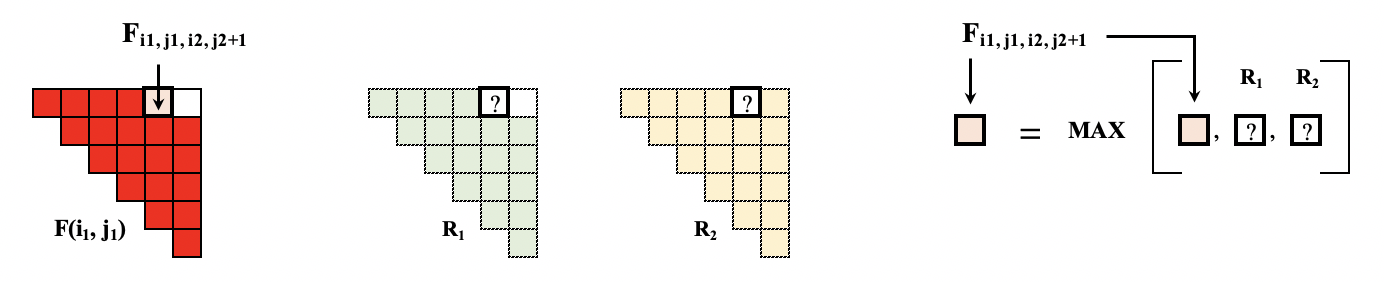
\includegraphics[scale=0.35, trim=4 4 4 4,clip]{content/figures/r0_r1_2.png}
\caption{Step 2: Next, we attempt to update $F_{i_{1}, j_{1}, i_{2}, j_{2} +1}$ highlighted in thick bordered light red box. 
%Results of $R^{0}$, $R^{3}$, and $R^{4}$ corresponding to this point is already available at $F_{i_{1}, j_{1}, i_{2}, j_{2} +1}$.  
$R^{1}$, and $R^{2}$ are not computed yet for $F_{i_{1}, j_{1}, i_{2}, j_{2} +1}$. Thus we need to compute these two reduction results before updating this point.}
\label{fig:r3_r4_2}
\end{subfigure}

\begin{subfigure}[htbp]{1\linewidth}
\centering
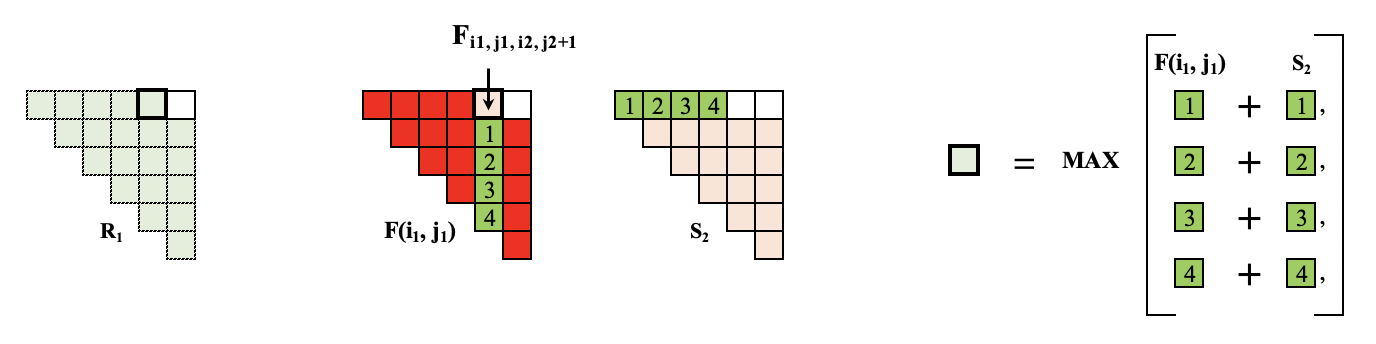
\includegraphics[scale=0.35, trim=4 4 4 4,clip]{content/figures/r0_r1_3.png}
\caption{Step 3: In this step, we compute  $R^{1}$ for $F_{i_1, j_1, i_2, j_2+1}$. It requires all the $F(i_1, j_1)$-table elements towards the south of $F_{i_1, j_1, i_2, j_2+1}$ and all the $S^{(2)}$-table elements towards the west of the corresponding $S^{(2)}$-table element.}
\label{fig:r3_r4_3}
\end{subfigure}


\begin{subfigure}[htbp]{1\linewidth}
\centering
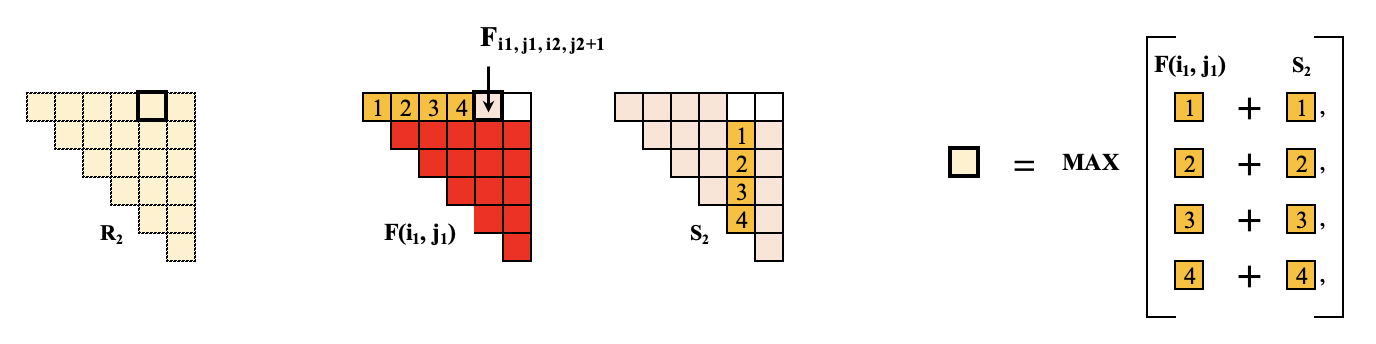
\includegraphics[scale=0.35, trim=4 4 4 4,clip]{content/figures/r0_r1_4.png}
\caption{Step 4: Now, we compute $R^{2}$ for  $F_{i_1, j_1, i_2, j_2+1}$. It requires all the $F(i_1, j_1)$-table elements towards the west of $F_{i_1, j_1, i_2, j_2+1}$ and all the $S^{(2)}$-table elements towards the south of the corresponding $S^{(2)}$-table element.}
\label{fig:r3_r4_4}
\end{subfigure}

\begin{subfigure}[htbp]{1\linewidth}
\centering
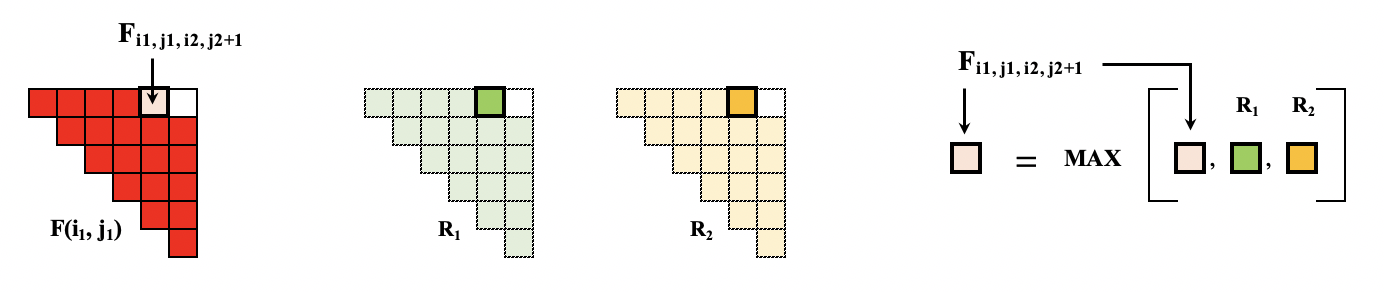
\includegraphics[scale=0.35, trim=4 4 4 4,clip]{content/figures/r0_r1_5.png}
\caption{Step 5: We have all the reduction results available at this point to update $F_{i_1, j_1, i_2, j_2+1}$. Next, we compute the $R^{1}$ and $R^{2}$ for updating the next $F$-table entry. This process continues until all the elements are updated.}
\label{fig:r3_r4_5}
\end{subfigure}
\caption{Illustration of $F$-table entry update with $R^{1}$ and $R^{2}$}
\label{fig:final_ftable_update}
\end{figure}
However, $R^3$ is an element-wise operation instead of the matrix product-like operations done in $R^{0}$. Similarly, $R^{4}$ can also be expressed as a set of element-wise max-plus operations between $S^{(1)}$ and $F$-table entries highlighted in Figure~\ref{fig:R_4_optimization}. After accumulating all the results from $R^{0}$, $R^{3}$, and $R^{4}$ into $F(i_{1}, j_{1})$, we updated it using $R^{1}$ and $R^{2}$. $R^{1}$ and $R^{2}$ have dependencies with the inner triangle that is being computed and $S^{(2)}$. Thus, these three updates must happen in a specific order demonstrated in Figure~\ref{fig:final_ftable_update}. Unlike $R^{0,3-4}$, we could not to tile these two reductions for each $F(i_{1}, j_{1})$. These are optimum string parenthesization (OSP)-like computations that require further transformation like middle serialization which were not trivial for our code generator. E.g., Simply pulling the reduction iteration($k_{2}$) from the innermost loop nest prohibits loop-tiling of the iteration space.

